\section{Architecture 3-tiers}
\label{ch:3-tiers}

\subsection{Présentation}

Dans le monde du développement informatique, un modèle d’architecture s’est imposé dans la réalisation d’application. Le modèle est appelé “Architecture trois tiers”. 
Il s’agit d’un modèle logique d’architecture applicative qui vise à modéliser une application en la divisant en trois couches.

Le but du 3 tiers est de séparer les 3 couches habituelles d’une application: IHM, traitements et données.
Une application sera composée de 3 couches indépendantes:

\begin{center}
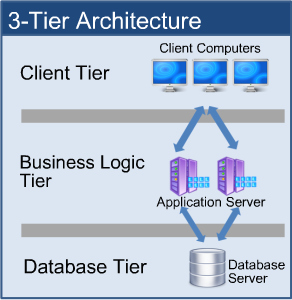
\includegraphics[scale=0.6]{img/3tier.jpg}
\label{Graphique technologie ajax}
\end{center}
 

\begin{list}{•}{}

  \item 
   La couche \textbf{présentation} des données : correspondant à la restitution et à l’affichage sur le clients, le dialogue avec l’utilisateur;
  
  \item
  Le \textbf{traitement} métier des données: correspondant à la mise en oeuvre de l'ensemble des règles de gestion et de la logique applicative;
  
  \item
  et enfin l’\textbf{accès aux données} persistantes : correspondant aux données qui sont destinées à être conservées sur la durée, voir de manière définitive   
  
\end{list}

Cette séparation a pour but de rendre indépendantes chacune des couches afin de simplifier la maintenance et les évolutions futures de l'application (par exemple, changement de système de base de données, portage d'un environnement graphique à un autre, ...).
Elle assure une sécurité plus importante car l'accès à la base de données n'est autorisé que par la couche Traitements.
Elle a également l'avantage d'optimiser le travail en équipe et de réduire les coûts de développement et de maintenance.

